\documentclass[12pt]{beamer}

\usetheme{Copenhagen}

\nonstopmode
% \usepackage{algorithm}
% % \usepackage{algcompatible}
% \usepackage{bm}
% \usepackage{bbm}
% \usepackage{algpseudocode}
% \usepackage{amsmath} % flere matematikkommandoer
% \usepackage{amssymb} % flere matematikkommandoer
% \usepackage{arydshln}
% \usepackage[utf8]{inputenc} % æøå
% \usepackage[T1]{fontenc} % mere æøå
% \usepackage{verbatim} % så man kan skrive ren tekst
% \usepackage[all]{xy} % den sidste (avancerede) formel i dokumentet
% \usepackage[margin=1in]{geometry}  % set the margins to 1in on all sides
% \usepackage{graphicx}              % to include figures
% \usepackage{amsfonts}              % for blackboard bold, etc
% \usepackage{amsthm}                % better theorem environments
% \usepackage{caption}
% \usepackage{bm}
% \usepackage{pgf}
% \usepackage{fancyhdr}
% \usepackage{hyperref}
% \usepackage{stmaryrd}
% \usepackage{mathtools}
% \usepackage{multirow}
\usepackage{listings}
% \usepackage{subcaption}
% \usepackage[inline]{enumitem}
% \usepackage[round]{natbib}
% \usepackage{breqn}
% \usepackage{tikz}
% \usetikzlibrary{arrows,automata,fit,positioning, shapes, calc, fadings}

% various theorems, numbered by section

\newtheorem{thm}{Theorem}[section]
\newtheorem{lem}[thm]{Lemma}
\newtheorem{prop}[thm]{Proposition}
\newtheorem{cor}[thm]{Corollary}
\newtheorem{conj}[thm]{Conjecture}

\DeclareMathOperator{\id}{id}
\DeclareMathOperator*{\argmin}{argmin}
\DeclareMathOperator*{\argmax}{argmax}

\newcommand{\nn}{\mathcal{N}}
\newcommand{\uu}{\mathcal{U}}
\newcommand{\bb}{\mathcal{B}}
\newcommand{\ee}{\mathrm{e}}
\newcommand{\rd}[1]{\mathrm{#1}}
\newcommand{\bd}[1]{\mathbf{#1}}  % for bolding symbols
\newcommand{\RR}{\mathbb{R}}      % for Real numbers
\newcommand{\ZZ}{\mathbb{Z}}      % for Integers
\newcommand{\PP}{\mathbb{P}}      % for Prob
\newcommand{\EE}{\mathbb{E}}      % for Expectation
\newcommand{\II}{\mathbbm{1}}      % for Indicator fun
\newcommand{\NN}{\mathbb{N}}      % for Prob
\newcommand{\col}[1]{\left[\begin{matrix} #1 \end{matrix} \right]}
\newcommand{\eqsys}[2]{ \left[\!\!
    \begin{array}{#1} #2
    \end{array}
    \!\!\right]}
\newcommand{\comb}[2]{\binom{#1^2 + #2^2}{#1+#2}}
\newcommand{\sint}[1]{\shortintertext{#1}}
\newcommand{\CTL}[1]{\:\textrm{#1}\:}
\newcommand{\sat}{\:\:\textrm{\textbf{sat}}\:\:}
\newcommand{\pr}{\textrm{Pr}}
\newcommand{\grw}{m_{\mathcal{H}}}
\newcommand{\dvc}{d_{VC}}
%\newtheorem{theorem}{Theorem}[section]
%\newtheorem{lemma}{Lemma}[theorem]
%\newtheorem{Lemma}{Lemma}[section]
%\newtheorem{corollary}{Corollary}[theorem]
% \newcommand{\lstbg}[3][0pt]{{\fboxsep#1\colorbox{#2}{\strut #3}}}
% \newcommand{\kl}{\textrm{kl}}
% \newcommand{\KL}{\textrm{KL}}
% \newcommand{\hyp}{\mathcal{H}}
% \lstdefinelanguage{diff}{
%   basicstyle=\ttfamily\scriptsize,
%   morecomment=[f][\lstbg{red!20}]-,
%   morecomment=[f][\lstbg{green!20}]+,
%   morecomment=[f][\textit]{@@},
%   %morecomment=[f][\textit]{---},
%   %morecomment=[f][\textit]{+++},
% }

% \newenvironment{gamedef}
% {%
%  \par\medskip\noindent    
%  \textbf{Game Defintion:} \\ % HEADLINE
%  \noindent For $t = 1,2,...$:
%     \begin{enumerate}[leftmargin=3em,labelsep=1em,beginpenalty=10000]
%     \setlength{\itemsep}{0.2em}
%     \setlength{\parskip}{0.5em}
%     \setlength{\parsep}{0pt}
% }
% {%
%     \end{enumerate}
% }
\definecolor{eclipseBlue}{RGB}{42,0.0,255}
\definecolor{eclipseGreen}{RGB}{63,127,95}
\definecolor{eclipsePurple}{RGB}{127,0,85}

% \DeclarePairedDelimiterX{\inp}[2]{\langle}{\rangle}{#1, #2}

\lstset{
  language={haskell},
  % basicstyle=\ttfamily, % Global Code Style
  % captionpos=b, % Position of the Caption (t for top, b for bottom)
  % extendedchars=true, % Allows 256 instead of 128 ASCII characters
  % tabsize=2, % number of spaces indented when discovering a tab
  % columns=fixed, % make all characters equal width
  % keepspaces=true, % does not ignore spaces to fit width, convert tabs to spaces
  % showstringspaces=false, % lets spaces in strings appear as real spaces
  % breaklines=true, % wrap lines if they don't fit
  % frame=trbl, % draw a frame at the top, right, left and bottom of the listing
  % frameround=tttt, % make the frame round at all four corners
  % framesep=4pt, % quarter circle size of the round corners
  % numbers=left, % show line numbers at the left
  % numberstyle=\small\ttfamily, % style of the line numbers
  % commentstyle=\slshape\bfseries\color{eclipseGreen}, % style of comments
  % keywordstyle=\bfseries\color{eclipsePurple}, % style of keywords
  % stringstyle=\color{eclipseBlue}, % style of strings
  % emphstyle=[1]{\color{eclipseBlue}},
  % moredelim=**[is][\color{red}]{@@}{@@}
}
\renewcommand{\thesubsubsection}{\thesection.\alph{subsubsection}}
\begin{document}
\author{Chi Pham \& William Sprent}
\title{Improving Rasterific}
\maketitle

\tableofcontents
\clearpage

\section{Introduction}
% Noget om hvad projektet går ud på, måske hovedresultater
\begin{frame}
  \begin{itemize}
  \item What
  \item Are
  \item We
  \item Talking
  \item Bout
  \end{itemize}
\end{frame}
\section{Background}\label{background}
\subsection{Rasterific}
\begin{frame}
\begin{figure}[h!]
  \centering
  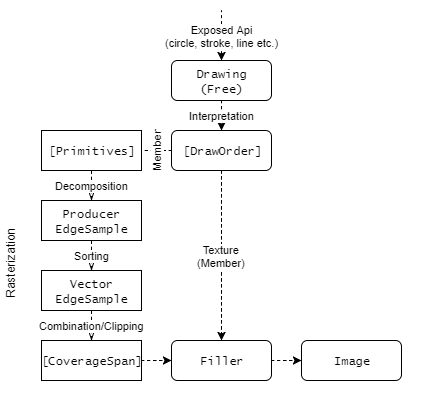
\includegraphics[width=.6\linewidth]{../rasterific-pipeline}
  \caption{Approximation of the Rasterific pipeline.}
  \label{fig:rasterific-pipeline}
\end{figure}
\end{frame}

\begin{frame}
\begin{enumerate}
\item the decomposition of primitives into \texttt{EdgeSample}s, a very fine-grained task with potential for constant span;
\item the sorting of \texttt{EdgeSample}s, a known problem with somewhat limited potential for parallism; and,
\item the combination of \texttt{EdgeSample}s into \texttt{CoverageSpan}s, a somewhat more complicated and course grained task with the highest potential for speedup at face value.
\end{enumerate}
\end{frame}
\section{Benchmarks}\label{sec:benchmarks}

\begin{frame}
\begin{itemize}
\item \textbf{Snowflake:} Draws a series of transparent snowflakes on a background. See Figure . Was added to the Rasterific project
   shortly before we started our project.
\item \textbf{BigSquare:} Draws a big pink snowflake (named for legacy reasons). We have added this to benchmark a single call to the rasteriser containing many \texttt{Primitives}. 
\item \textbf{Lines:} Draws a large number of randomly colored lines on a background. 
  We have added this to benchmark line primitive decomposition.
\end{itemize}
\end{frame}
\begin{frame}
\begin{figure}[h!]
  \centering
  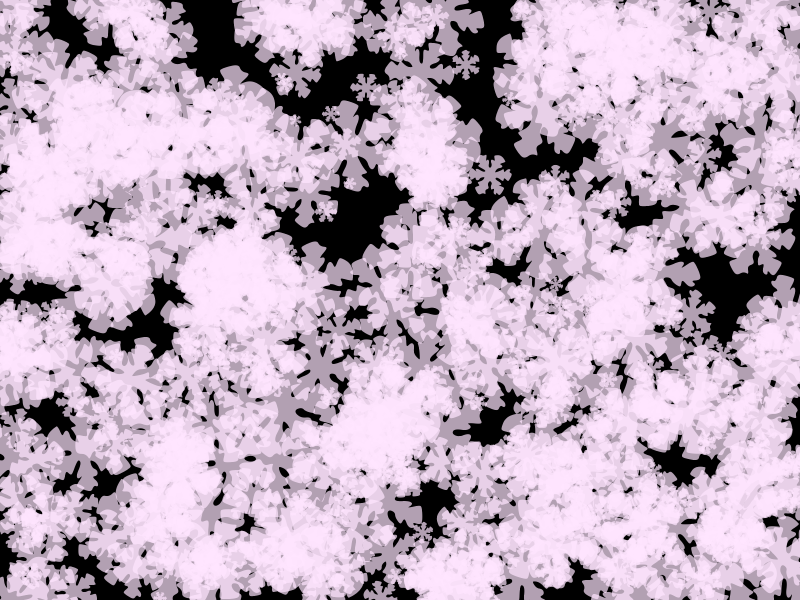
\includegraphics[width=.4\linewidth]{../flakes}
  \caption{The result of the ``snowflake'' benchmark.}
  \label{fig:snowflakes}
\end{figure}
\end{frame}

\begin{frame}
\begin{figure}[H]
  \centering
  
\includegraphics[width=.2\linewidth]{../bigsquare}
  \caption{The output of the \texttt{bigsquare} benchmark.}
  \label{fig:bigsquare-benchmark}
\end{figure}
\end{frame}

\begin{frame}
\begin{figure}[H]
  \centering
  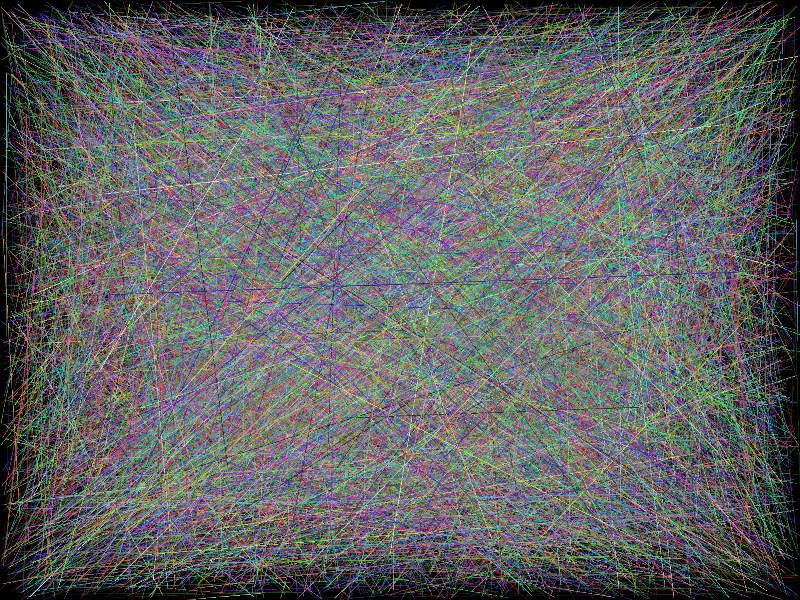
\includegraphics[width=.4\linewidth]{../lines}
  \caption{The output of the \texttt{lines} benchmark.}
  \label{fig:lines-benchmark}
\end{figure}
\end{frame}

\section{Experiments}\label{experiments}

\begin{frame}
\begin{figure}[H]
  \centering
  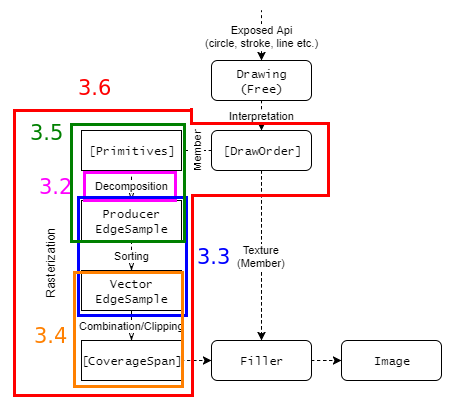
\includegraphics[width=.6\linewidth]{../rasterific-pipeline-flot}
  \caption{Parallelisation granularity in the Rasterific pipeline.}
  \label{fig:rasterific-pipeline-flot}
\end{figure}
\end{frame}


\begin{frame}
  How primitives are decomposed
\end{frame}


\begin{frame}
\begin{figure}[h!]
  \centering
  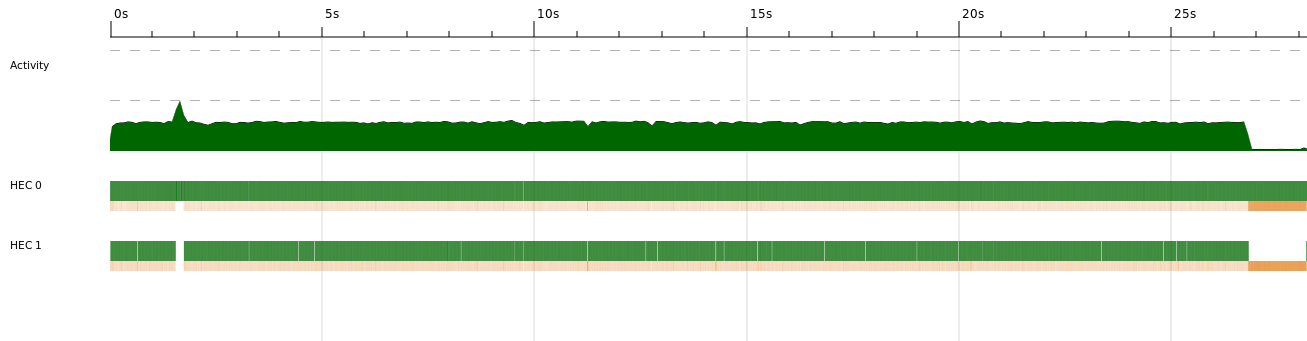
\includegraphics[width=0.85\linewidth]{../threadscope/lines/single-split}
  \caption{ThreadScope output for parallelising line decomposition. Shows the output for the
    \texttt{lines} benchmark.}
  \label{fig:line-thread}
\end{figure}

\begin{figure}[h!]
  \centering
  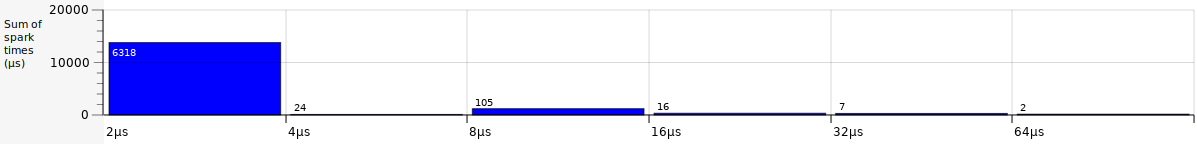
\includegraphics[width=0.85\linewidth]{../threadscope/lines/single-split-spark-times}
  \caption{ThreadScope spark times for Figure }
  \label{fig:line-thread-sparks}
\end{figure}
\end{frame}


\begin{frame}
\begin{figure}[h!]
  \centering
  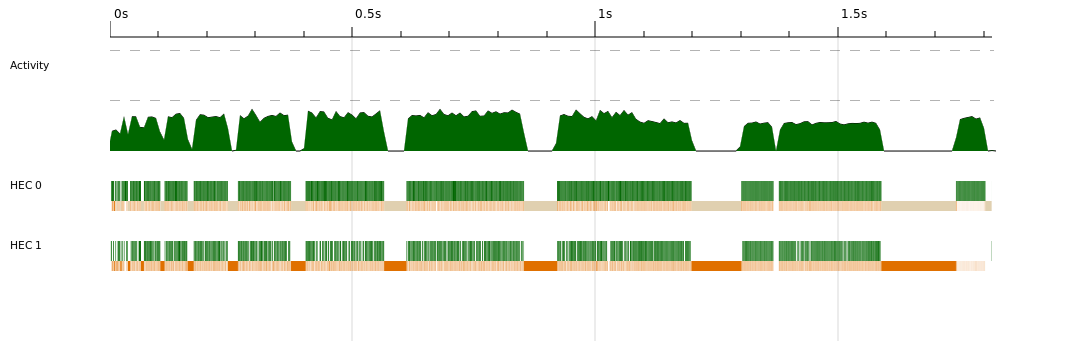
\includegraphics[width=0.85\linewidth]{../threadscope/lines/single-line-every-10}
  \caption{ThreadScope output for running line decomposition on a single line with length
    100000.}
  \label{fig:single-line-thread}
\end{figure}

\begin{figure}[h!]
  \centering
  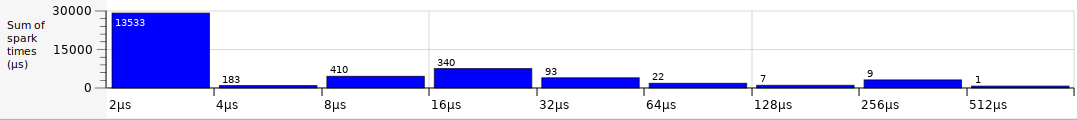
\includegraphics[width=0.85\linewidth]{../threadscope/lines/single-line-every-10-spark-times}
  \caption{ThreadScope output for running line decomposition on a single line with length
    100000.}
  \label{fig:single-line-thread-sparks}
\end{figure}
\end{frame}

\begin{frame}
 \begin{figure}[h!]
  \centering
  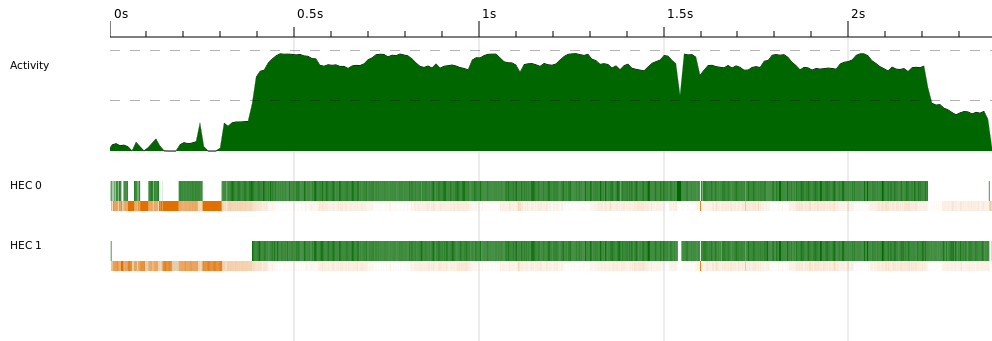
\includegraphics[width=0.85\linewidth]{../threadscope/sorting/sorting-final}
  \caption{ThreadScope output for sorting 1.000.000 \texttt{EdgeSample}s.}
  \label{fig:sorting-thread}
\end{figure}

 \begin{figure}[h!]
  \centering
  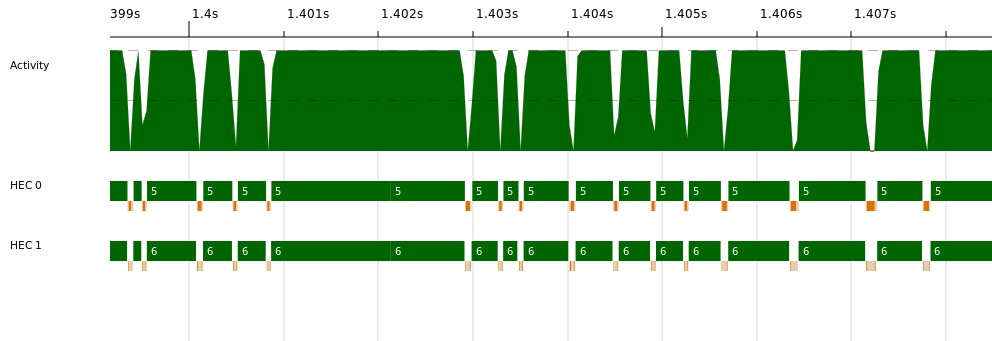
\includegraphics[width=0.85\linewidth]{../threadscope/sorting/sorting-final-zoom}
  \caption{ThreadScope output for sorting 1.000.000 \texttt{EdgeSample}s.}
  \label{fig:sorting-thread-zoomed}
\end{figure}
\end{frame}

\begin{frame}
\begin{figure}[h!]
  \centering
  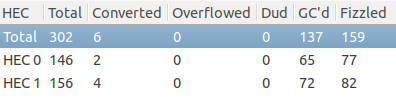
\includegraphics[width=0.6\linewidth]{../threadscope/sorting/sorting-final-sparks}
  \caption{ThreadScope spark output for sorting 1.000.000 \texttt{EdgeSample}s.}
  \label{fig:sorting-thread-sparks}
\end{figure}
 \begin{figure}[h!]
  \centering
  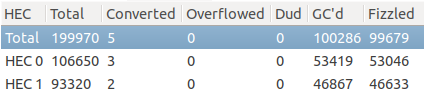
\includegraphics[width=0.6\linewidth]{../threadscope/sorting/sorting-100k-sparks}
  \caption{ThreadScope spark output for sorting 100.000 \texttt{EdgeSample}s!}
  \label{fig:sorting-thread-100k-sparks}
\end{figure}
\end{frame}

\begin{frame}[fragile]
  \begin{large}
    text
  \end{large}
\end{frame}

\begin{frame}
 \begin{figure}[H]
  \centering
  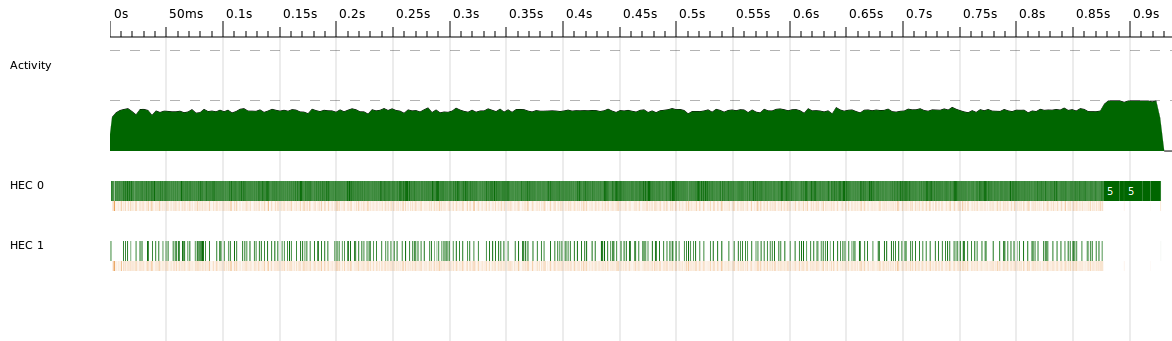
\includegraphics[width=\linewidth]{../threadscope/combinegrouped/bigflake}
  \caption{ThreadScope output for running the \texttt{snowflake} program with 500 snowflakes.}
  \label{fig:combinegrouped}
\end{figure}

 \begin{figure}[H]
  \centering
  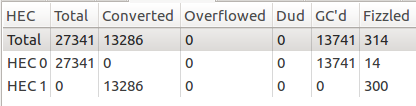
\includegraphics[scale=1]{../threadscope/combinegrouped/sparks}
  \caption{ThreadScope spark output for running the \texttt{snowflake} program with 500 snowflakes.}
  \label{fig:combinegrouped-sparks}
\end{figure}
\end{frame}


\begin{frame}
 \begin{figure}[h!]
  \centering
  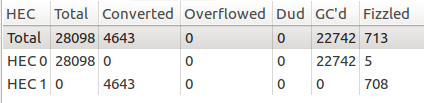
\includegraphics[scale=1]{../threadscope/combineindex/sparks}
  \caption{ThreadScope spark output for running the \texttt{snowflake} program with 500 snowflakes.}
  \label{fig:combineindex-sparks}
\end{figure}
\end{frame}

\begin{frame}
  \begin{itemize}
  \item Some
  \item Text
  \item maybe
  \end{itemize}
\end{frame}

\begin{frame}
 \begin{figure}[H]
  \centering
  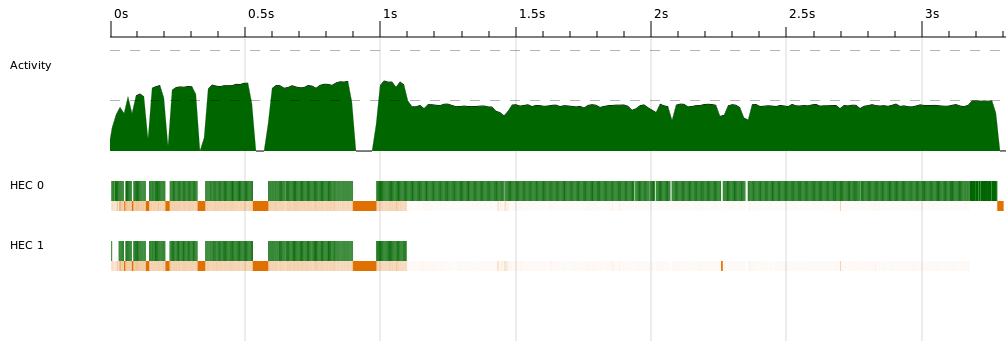
\includegraphics[width=\linewidth]{../threadscope/fillorder/lines}
  \caption{ThreadScope output for running the \texttt{lines} program with 5000 lines.}
  \label{fig:lines-fillorder}
\end{figure}

\begin{figure}[H]
  \centering
  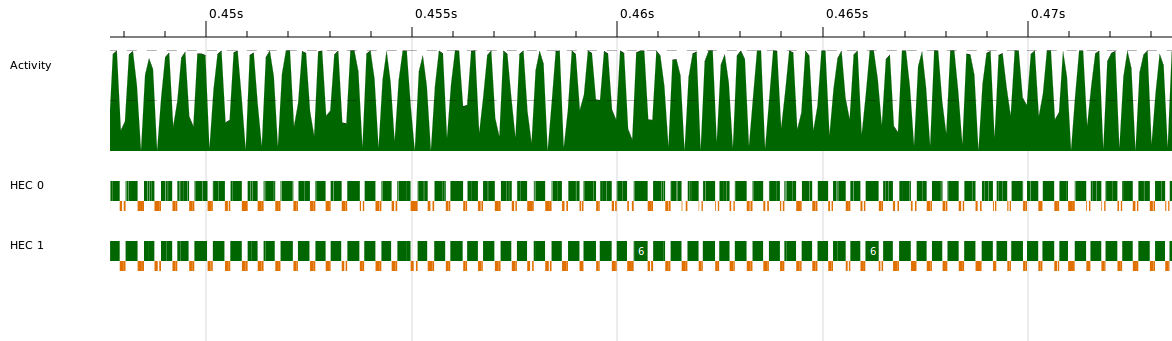
\includegraphics[width=\linewidth]{../threadscope/fillorder/lines-zoom}
  \caption{Zoomed ThreadScope output for running the \texttt{lines} program with 5000 lines.}
  \label{fig:lines-fillorder-zoom}
\end{figure}

\end{frame}

\begin{frame}
 \begin{figure}[H]
  \centering
  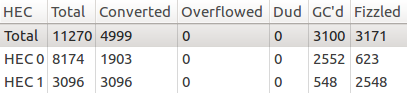
\includegraphics[scale=1]{../threadscope/fillorder/lines-spark}
  \caption{ThreadScope spark output for running the \texttt{lines} program with 5000 lines.}
  \label{fig:lines-fillorder-spark}
\end{figure}


 \begin{figure}[H]
  \centering
  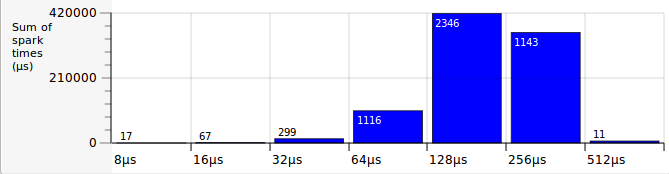
\includegraphics[scale=0.7]{../threadscope/fillorder/lines-spark-sizes}
  \caption{ThreadScope spark sizes output for running the \texttt{lines} program with 5000 lines.}
  \label{fig:lines-fillorder-sizes}
\end{figure}
\end{frame}


\subsection{Results}

\begin{frame}
\begin{table}[h!]
  \centering
  \begin{tabular}[h!]{|r|c|c|c|}\hline
    & \multicolumn{3}{|c|}{\textbf{Benchmark}} \\
    \textbf{Version}&\textbf{Lines}&\textbf{Snowflake}&\textbf{Bigsquare} \\\hline
    Sequential & 572.6 ms & 740.4 ms & 179.3 ms \\
    FillOrder () &  575.4 ms & 769.8ms & 183.3ms \\
    Sorting () &970.8ms& 1.061 s & 205.2 ms \\
    Combine () & 777.9 ms & 862.1 ms & 214.2 ms \\
    Combine () & 769.8 ms & 877.3 ms & 198.5 ms \\\hline
  \end{tabular}                                       
  \caption{Benchmark results on the various parallisations made above. Parallel version were run with
   \texttt{+RTS -N2}, that is on two cores.}                         
  \label{tab:benchmark-results}
\end{table}
\end{frame}

\section{Discussion}\label{discussion}

\begin{frame}
  \begin{itemize}
  \item bullet
  \item points
  \end{itemize}
\end{frame}
\begin{frame}
\begin{figure}[H]
  \centering
  \begin{tabular}{|c|c|c|c|c|}
  \hline
  \textbf{Benchmark} & \texttt{DrawOrder} & \texttt{Primitive} & \texttt{EdgeSample} & \texttt{CoverageSpan} \\\hline
  \texttt{snowflake} & 500 & 148 & 1733 & 1427 \\\hline
  \texttt{bigsquare} & 1 & 148 & 103626 & 90142 \\\hline
  \texttt{lines} & 1000 & 1 & 1916 & 1375 \\\hline
  \end{tabular}
  \caption{Maximum numbers of elements of each type, being parallelised in the three benchmarks.}
  \label{fig:bench-numbers}
\end{figure}
\end{frame}
% Perhaps use this link somewher https://www.reddit.com/r/haskell/comments/747zx1/parallel_computation_in_st/


\section{Further Work}\label{furtherwork}
\begin{frame}
\begin{itemize}
\item Shift Rasterific from relying on laziness, and try to unify which data strucures are used throughout the library to make it more easy to construct
  broad parallel solutions. Perhaps take a look at the Repa package.
\item Try to flatten the calls into the inner rasterization pipeline. This could perhaps enable more course grained parallelism which could be more readily exploited.
  This may require changes to the public API, but may be worth it.
\item While not fully related, we stumbled on to a discussion\footnote{\url{https://www.reddit.com/r/haskell/comments/747zx1/parallel_computation_in_st/}}
  about parallel in-place sorting in Haskell using the ST monad.
  It would be interesting to try to implement a parallel sorting library and see if it is worth it.
  
\item Even for smaller modular attempts at parallelising, our efforts are not exhaustive. There are other places where it could be applied, such as for clipping, which is done just before rasterising. The clipping functions actually return difference lists and so would be much cheaper to concatenate, once computed.
\end{itemize}
\end{frame}
\section{Conclusion}
\begin{frame}
??
\end{frame}
\end{document}
